\documentclass[conference]{IEEEtran}
\usepackage{cite}
\usepackage{amsmath,amssymb,amsfonts}
\usepackage{algorithmic}
\usepackage{graphicx}
\usepackage{textcomp}
\usepackage{xcolor}
\def\BibTeX{{\rm B\kern-.05em{\sc i\kern-.025em b}\kern-.08em
    T\kern-.1667em\lower.7ex\hbox{E}\kern-.125emX}}
\begin{document}

\title{Vision and Cognitive Systems Final Project}
\author{\IEEEauthorblockN{Fabio Polito}
\IEEEauthorblockA{\textit{230635@studenti.unimore.it}}
\and
\IEEEauthorblockN{Giordano Costi}
\IEEEauthorblockA{\textit{226934@studenti.unimore.it}}\\
\large{Univerisity of Modena and Reggio Emilia}
\and
\IEEEauthorblockN{Stefano Carretti}
\IEEEauthorblockA{\textit{227250@studenti.unimore.it}}
}
\maketitle


\section{Introduction}
In this paper, we present a method to detect and identify paintings starting from a video taken inside “Galleria Estensi, Modena”.\\
Each frame is processed with image processing techniques in order to localize paintings, rectify distortions, and fetch from the database the corresponding work of art.\\
At the same time, an artificial neural network (YoloV3) detects people, which are localized inside a room of the museum.

\section{Related Works}
To remove camera noise but maintains the contours a  Bilateral filter\cite{b1} is used.
OTSU\cite{b2} is an automatic thresholding method widely used when the numbers of pixels in each class are close to each other.
Opencv Find Counturs\cite{b3} function is been used to find counturs in a previouslly modified frame in order to detect painting
The functions approxPolyDP\cite{b4} approximate a curve or a polygon with another curve/polygon with less vertices so that the distance between them is less or equal to the specified precision. It uses the Douglas-Peucker algorithm  
ORB\cite{b5} is a feature detection algorithm like SIFT while being almost two orders of magnitude faster.
YoloV3 \cite{b5}  is a famous neural network for fast object detection, will be used in this paper for people detection

\section{Painting Detection}
All frames are exctracted in sequence from the video and processed independently. The followed pipeline is explained afterwards.

\subsection{Preprocessing}
First of all, each frame is converted into black and white and processed with a bilateral filter to remove noise while preserving at the same time the edges.\\
After that, we apply otsu threshold  with the aim to separate the pixels into background and paintings, due to their chromatic difference.

\subsection{Bounding Box detection}
Using the function findContours of OpenCV, we obtain the outlines of the objects in the foreground, among which there will also be the paintings that we are looking for.\\
We then create the bounding box containing this contours and to eliminate the rectangles identified inside the paintings, we keep only the external ones and eliminate those contained within others.\\
Among the remaining bounding boxes, those that are not judged as paintings by an SVM model, will get discarded.

\subsection{SVM}
To classify the ROI proposed by the previous pipeline, an SVM model is been trained.\\
The algorithm takes as input the concatenation of the three histograms, one for each color plane.\\
The training dataset is composed of 1025 instances taken from bounding boxes derivate from the videos inside the museum and manually labeled.
409 of the samples are labeled as holding a painting and 604 as inaccurate bounding box.\\
A radial basis function kernel is been exploited for the classification.
The model returns False if the rectangle doesn't contain a painting and True if it does.



\subsection{Precision boosting and paintings segmentation}
To obtain a better segmentation within each bounding box we apply a further refinement of the images.\\
Observing the low light in the videos that were provided to us, the paintings\\
are significantly darker compared to their frame and do not correspond to the brightness of the paintings in the database. This leads to poor precision in the retrieval step. To cope with this problem, the brightness component is increased for each previously found bounding box.\\
Afterward, by transforming its format from BGR to HSV and then applying the otsu threshold again, we are able to obtain a more precise distinction between painting and frame/background, which will then be used during the retrieval and rectification steps.


\section{Painting Retrieval}
For the retrieval of the paintings situated in the database we use an approach based on feature detection algorithms.\\ 
After consulting a paper that performs a comparative analysis between the most well known algorithms ~\cite{b1} to get a general idea of the strengths and weaknesses of the different methods available to us, we carried out some experiments focusing on SIFT, AKAZE and ORB.\\
The results obtained made us opt for ORB, because overall it gave us more precise results than AKAZE and, unlike SIFT, it’s free of charge, therefore usable without fees in a possible commercial application.\\
To save time, the key points of the paintings in the database have been previously calculated and stored using the pickle module [link pickle documentation].\\
It implements binary protocols for serializing and de-serializing a Python object structure.\\
This data is loaded only once during the launch of the program.
The key points are computed from the bounding boxes detected by the previously described pipeline and afterward, to determine the best matches, the ratio test proposed by D. Lowe in the SIFT paper is performed[Reference to the sift paper].\\
This measure is obtained by comparing the distance of the closest neighbor to that of the second-closest neighbor.\\
This measure performs well because correct matches need to have the closest neighbor significantly closer than the closest incorrect match to achieve reliable matching.\\

\begin{figure}[htbp]
\centerline{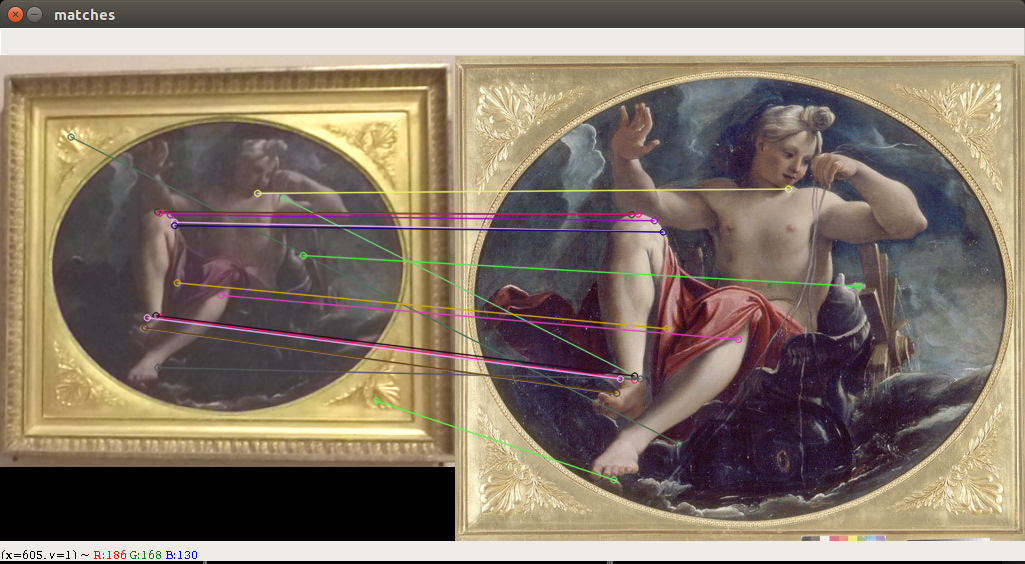
\includegraphics[width=0.8\columnwidth]{../Orb_matches/match3.png}}
\caption{Orb matches}
\label{fig_Orb_matches}
\end{figure}

For false matches, there will likely be a number of other false matches within similar distances due to the high dimensionality of the feature space.\\
In our implementation we reject all matches in which the distance ratio is greater than 0.75.\\
This allows us to keep the number of correctly retrieved paintings still high but at the same time to decrease the number of false positive.
A ranking with the 5 best matches found is then created and saved to a CSV file to show the results.\\
To understand if the painting is actually recognized among those in the DB, the average of the key points matched among the best 5 ranked is calculated and, if the first one differs from it for more than significant value, it is considered as correct and shown on the interface.


\section{Painting Rectification}
\subsection{Four points transform}
On the contour found with the techniques described in \textbf{Precision boosting and paintings segmentation} is applied the function approxPolyDP from OpenCV to approximate it to a polygonal curve.\\
If the shape returned has four vertices we can assume that the process has found a rectangular painting.\\
Given the four points, we are able to estimate the homography and apply the transformation to rectify the painting.\\
To calculate the aspect ratio for the projected rectangle we use an implementation based on this paper [] which derives the equations assuming a pinhole camera model.\\
This pipeline is applied to the paintings that don't get a match on the database.

\begin{figure}[htbp]
\centerline{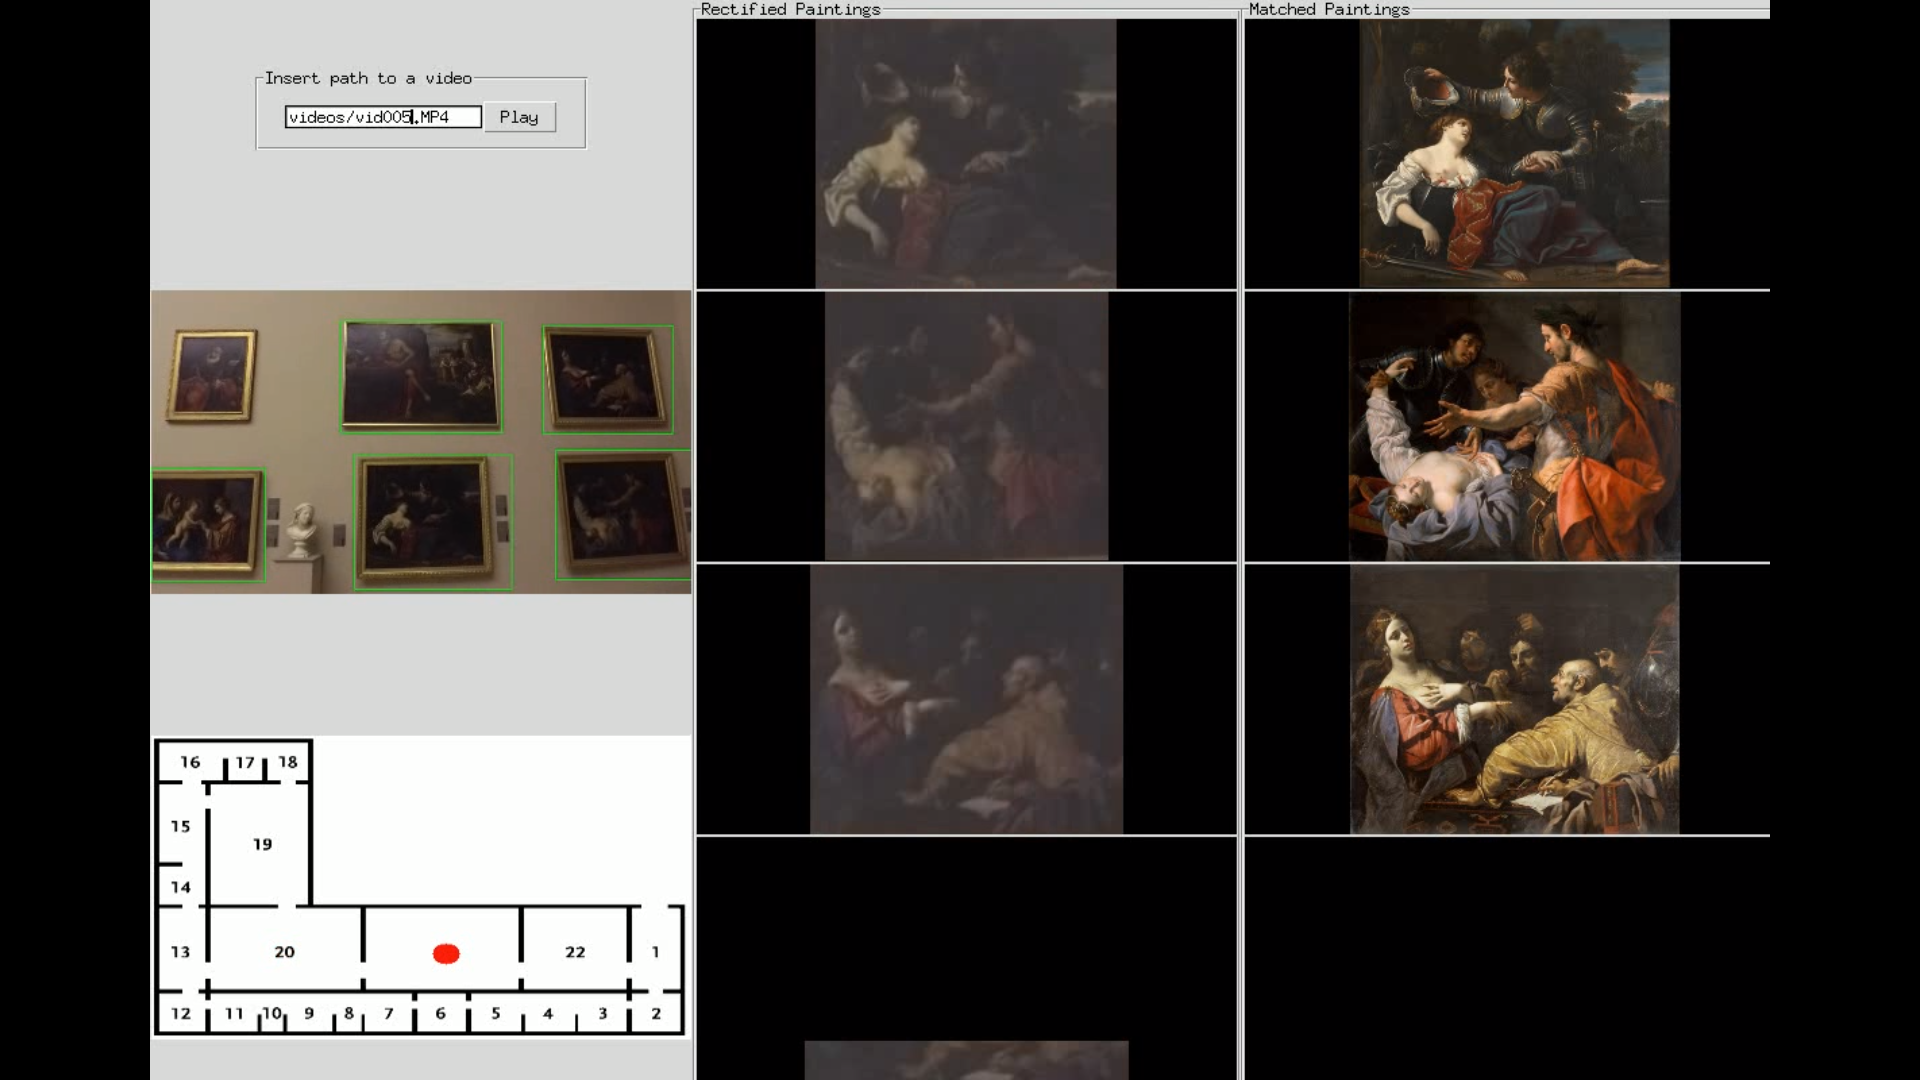
\includegraphics[width=0.8\columnwidth]{../detection_and_rectification/top_association_vid05.png}}
\caption{Painting detection and rectification}
\label{fig_Painting_detection_and_rectification}
\end{figure}

\subsection{alignImages}
Not all the paintings inside the museum have a rectangular shape. This means that the approximation found by approxPolyDP does not consist of 4 vertices, making the method just explained impractical.\\
The approach that is used in this case is based on the common keypoints found between the distorted image and the corresponding match in the database.\\
Through ORB feature matching algorithm the key points are computed from each bounding boxes detected by the previous pipeline and subsequently, to determine the best matches between it and the images of the database, the ratio test is used.\\
From them we calculate the homography matrix and
to avoid mismatches, the RANSAC algorithm is exploited.\\
To obtain a better result also the inverse warping algorithm is utilized.

\section{People Detection}
A neural network (YoloV3) is used for people detection.\\
At inference time each video frame is passed through the network that find all bounding boxes containing one of the objects in our classes list.\\
The weights for the network are obtained from an already trained network on COCO[ reference to COCO paper], a famous dataset containing 80 different classes.\\
In our case the only wanted class is the person one, for ease of use the network has not been modified, but from its output will be deleted all the classes with an id different from 0 that is the id of the person class.\\

\begin{figure}[htbp]
\centerline{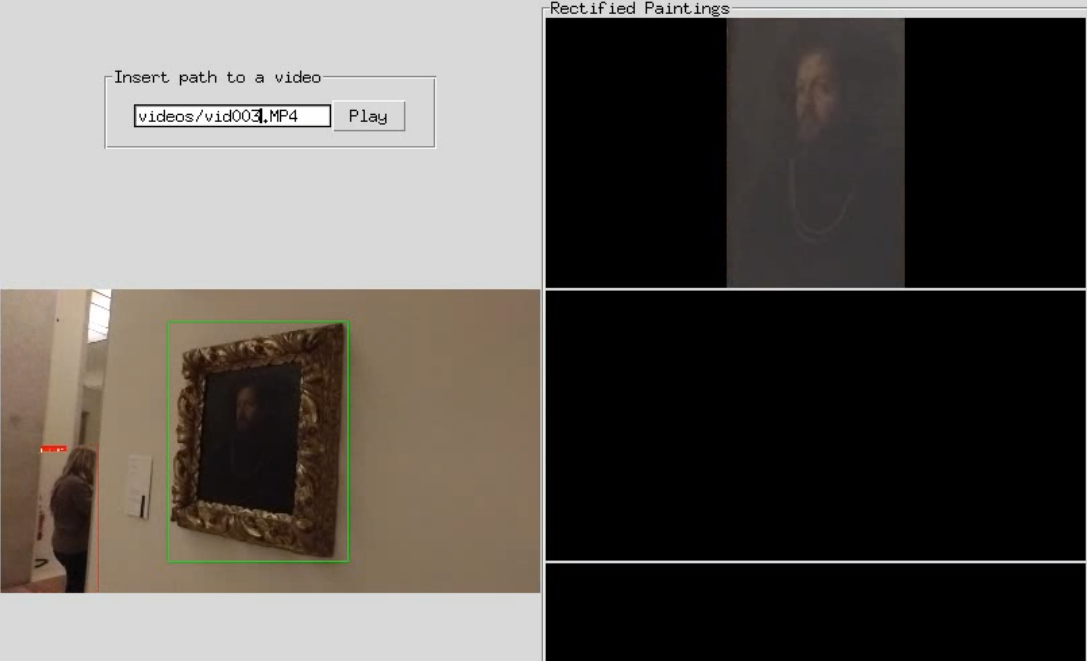
\includegraphics[width=0.8\columnwidth]{../people_detection/paint_and_person.png}}
\caption{People detection}
\label{fig_People_detection}
\end{figure}

A little problem has arisen due to the high number of paintings representing persons, in fact the network detect them also inside the paintings, to prevent these false positive we added a new control on the pixel position in order to cut out all the people detected inside a bounding box previously classified as a painting.

\begin{figure}[htbp]
\centerline{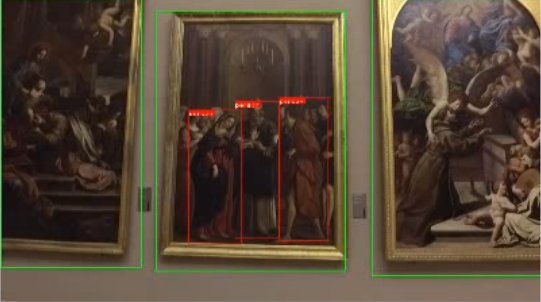
\includegraphics[width=0.8\columnwidth]{../people_detection/people_error.png}}
\caption{People detection error}
\label{fig_People_detection_error}
\end{figure}

\begin{figure}[htbp]
\centerline{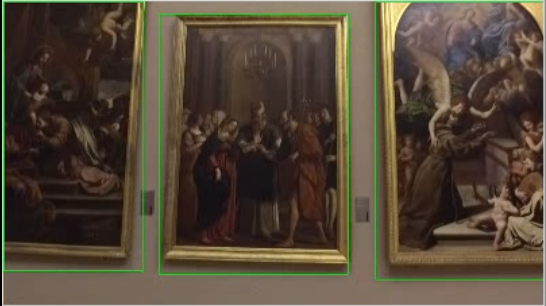
\includegraphics[width=0.8\columnwidth]{../people_detection/people_error_fixed.png}}
\caption{People detection error fixed}
\label{fig_People_detection_error_fixed}
\end{figure}

\section{People Localization}
Starting from a previously detected and retrieved painting from the database, we search the corresponding room in csv file, then a little red dot is printed on the museum image map. With this method we assume that all the painting detected and the persons are in the same room.
Moreover the localization will work only if the painting matched is considered safe that means the painting need to have a good level of matches, otherwise localization is not active.

\section{Painting Replacement in the 3D Model}
The pipeline followed to accomplish this task is similar to the one explained before with a little difference. we start directly with the hsv version of the image taken as input (a screenshot from the 3d model); then we apply Otsu threshold, followed by noise removal thanks to opening or closing process, keeping the one that maximizes the number of contours found. At this point we loop over each contour and find an approximation of itself with approxPolyDP; if the approximation has a shape described by 4 vertices, we estimate keypoints with orb and fetch the corresponding image from the database. Once this is done, if the image fetched is judged as a good match, we align that image with respect to the screenshot’s image plane and superimpose the result on the input image.

\begin{figure}[htbp]
\centerline{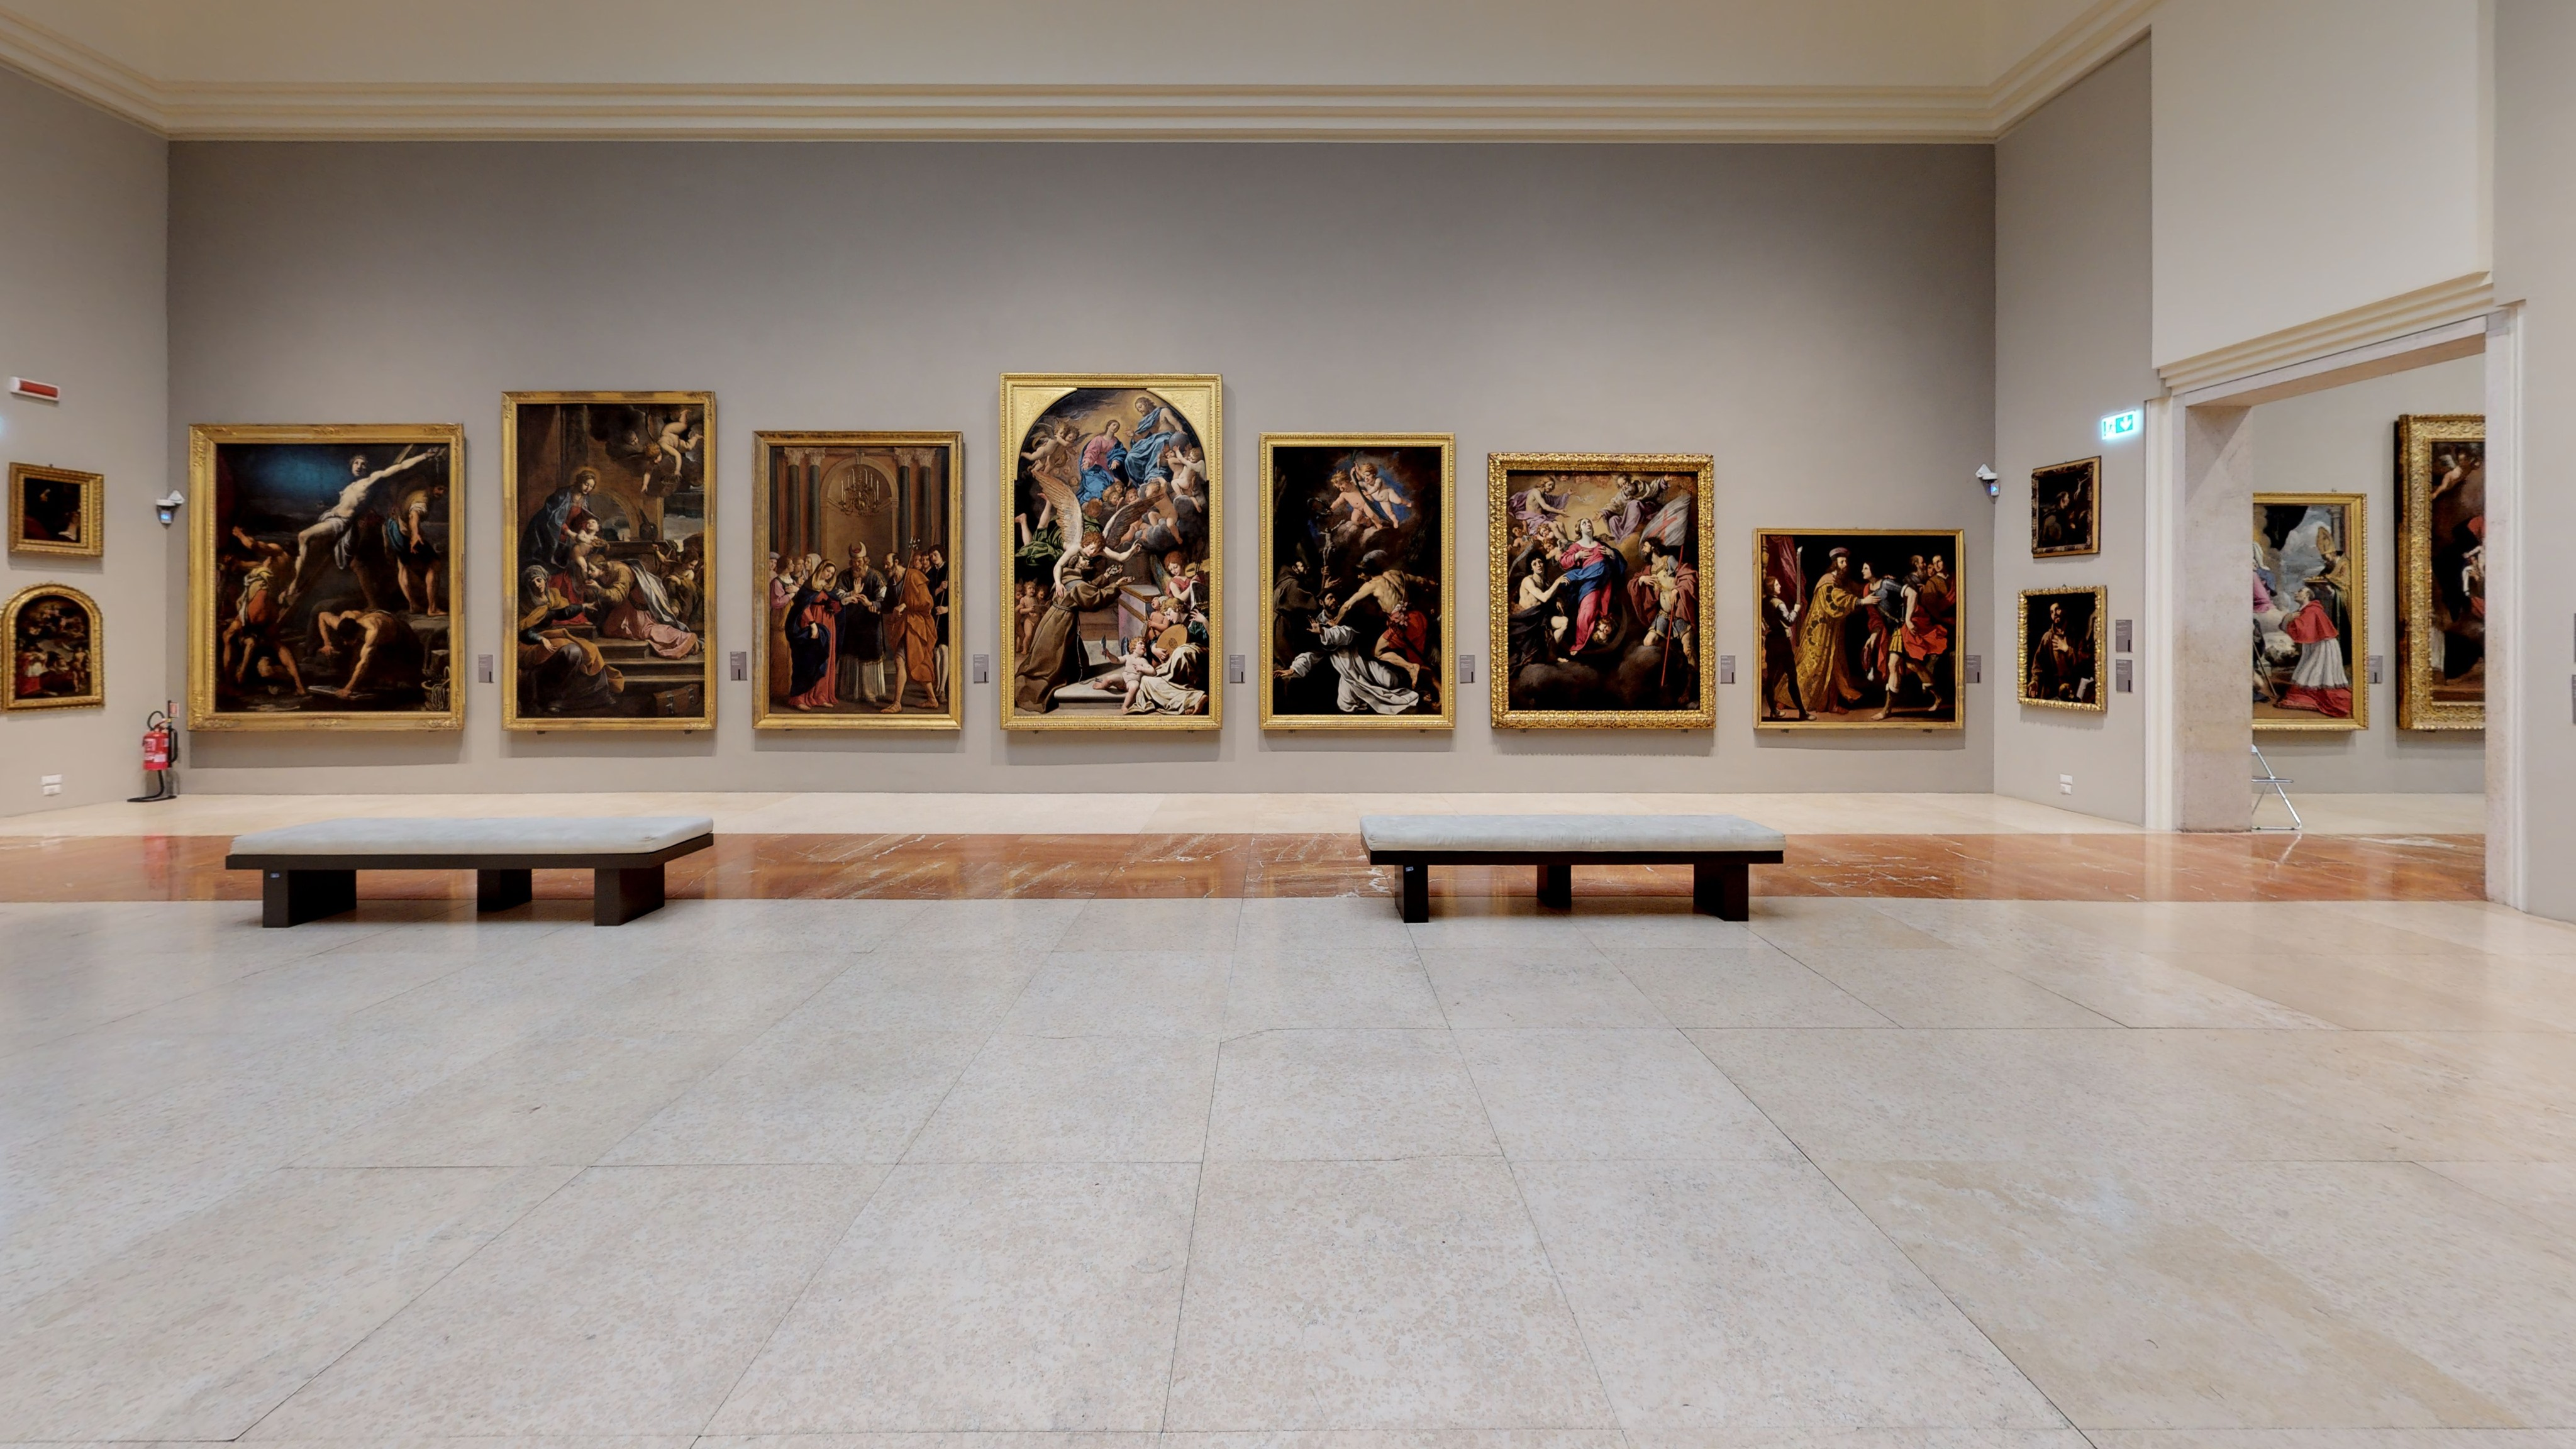
\includegraphics[width=0.8\columnwidth]{../screenshots_3d_model/screenshot_01.jpg}}
\caption{3dmodel}
\label{fig_3d_model}
\end{figure}

\begin{figure}[htbp]
\centerline{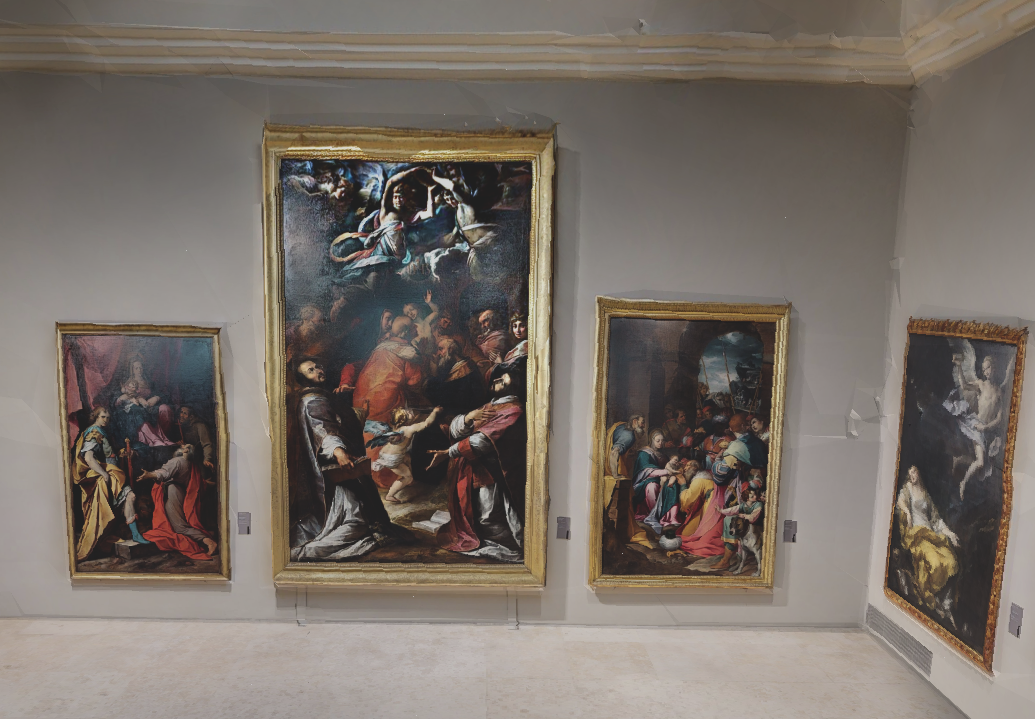
\includegraphics[width=0.8\columnwidth]{../screenshots_3d_model/screenshot_03.png}}
\caption{3d model 2}
\label{fig_3d_model_2}
\end{figure}

What is worth to mention is that the alignment function that we use in this process is the same of the main pipeline of painting rectification. this function in fact takes as input two images and project the first one on the plane of the second. if the second image is a painting fetched from the database, it means that the first image is rectified; if instead the second image is a painting coming from a frame/screenshot, it means that we want to distort an image in order to match the perspective of that painting.



\section{Metrics and Precision}
To calculate the precision of the presented method we took almost 10 random frame for 6 different videos and labeled all the paintings by hand using a tool for labeling (normally used for yolo labels). Then with a custom code we calculated precision recall… comparing hand made labels with automatically generated ones.

\begin{figure}[htbp]
\centerline{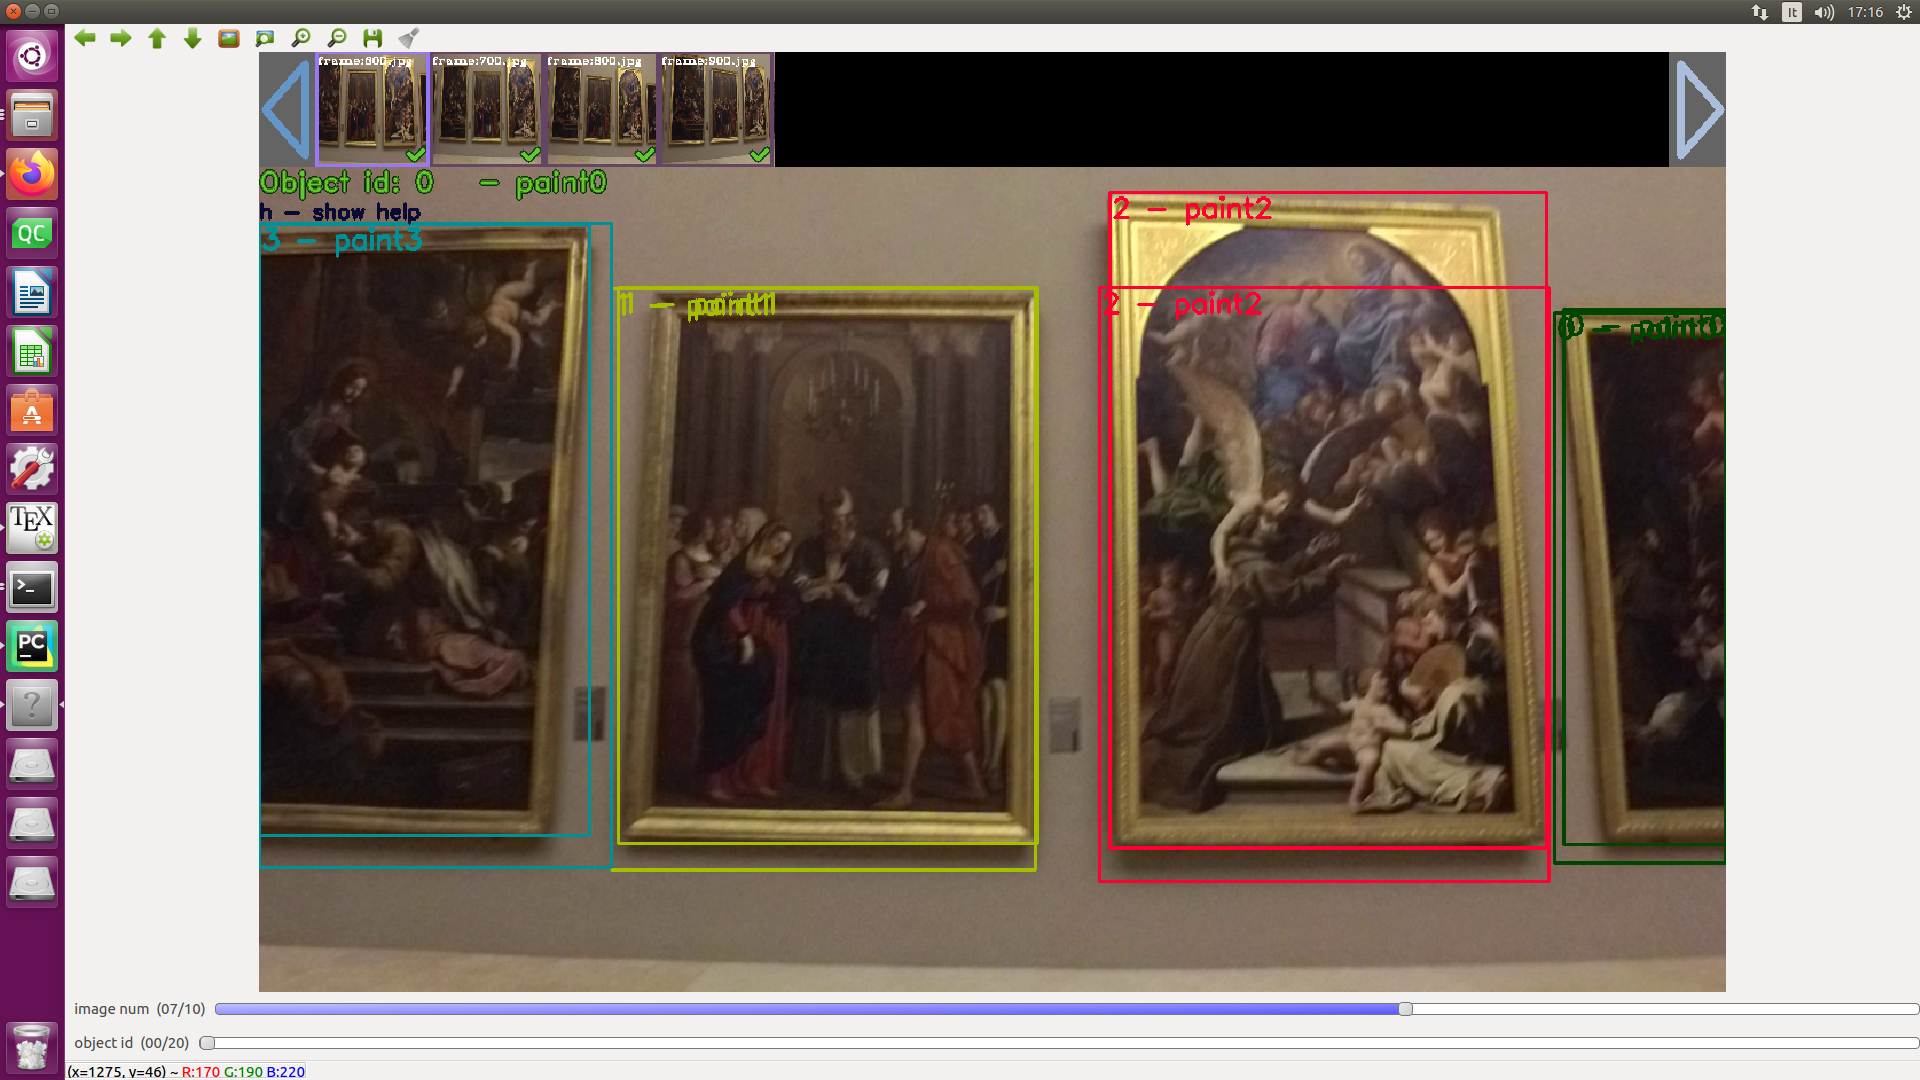
\includegraphics[width=0.8\columnwidth]{../Labeling_precision_metrics/Precision_Labeling.png}}
\caption{labeling}
\label{fig_labeling}
\end{figure}

\begin{table}[htbp]
\caption{Metrics Table}
\begin{center}
\begin{tabular}{|c|c|c|c|}
\hline
\textbf{Table}&\multicolumn{3}{|c|}{\textbf{Table Column Head}} \\
\cline{2-4} 
\textbf{Head} & \textbf{\textit{Table column subhead}}& \textbf{\textit{Subhead}}& \textbf{\textit{Subhead}} \\
\hline
copy& More table copy$^{\mathrm{a}}$& &  \\
\hline
\multicolumn{4}{l}{$^{\mathrm{a}}$Sample of a Table footnote.}
\end{tabular}
\label{tab1}
\end{center}
\end{table}


\section{Discussions}
Our approach is based on the assumption that input videos contain a relevant chromatic difference between paintings and background. when this assumption doesn’t occur, for example in the case of a wider shot comprising hallway too, otsu doesn’t manage to correctly differentiate paintings from the rest, which leads to worse performances.

\subsection{tested methods history}
At the beginning the idea was to use Canny, preceded by an initial noise removal obtained by bilateral filter, in order to find the edges on which to apply findContours opencv function. The results were not entirely satisfactory as the outlines often produced by canny did not accurately identify the picture. We therefore opted for a solution based on the thresholding of the RGB image, which as already explained above is followed by a refinement carried out at the hsv level. A method based only on hsv images was also tested, which revealed to be very performing in certain situations (in each frame there is a clear distinction between picture and background) but less stable than the previously exposed method.
It was then necessary to face the fact that each method, being based solely on image processing techniques, produced many false positives. The simplest way, according to which only bounding boxes containing a painting that had been matched on the database should have been shown, was discarded due to the limited database. many correctly identified paintings were in fact discarded because they were not present in the database. The solution adopted was to train an svm with the goal to classify what is a painting and what is not.



\section{References}
Please number citations consecutively within brackets \cite{b1}. The 
sentence punctuation follows the bracket \cite{b2}. Refer simply to the reference 
number, as in \cite{b3}---do not use ``Ref. \cite{b3}'' or ``reference \cite{b3}'' except at 
the beginning of a sentence: ``Reference \cite{b3} was the first $\ldots$''

Number footnotes separately in superscripts. Place the actual footnote at 
the bottom of the column in which it was cited. Do not put footnotes in the 
abstract or reference list. Use letters for table footnotes.

Unless there are six authors or more give all authors' names; do not use 
``et al.''. Papers that have not been published, even if they have been 
submitted for publication, should be cited as ``unpublished'' \cite{b4}. Papers 
that have been accepted for publication should be cited as ``in press'' \cite{b5}. 
Capitalize only the first word in a paper title, except for proper nouns and 
element symbols.

For papers published in translation journals, please give the English 
citation first, followed by the original foreign-language citation \cite{b6}.

\begin{thebibliography}{00}
\bibitem{b1} C. Tomasi and R. Manduchi, "Bilateral filtering for gray and color images," Sixth International Conference on Computer Vision (IEEE Cat. No.98CH36271), Bombay, India, 1998, pp. 839-846, doi: 10.1109/ICCV.1998.710815..
\bibitem{b2} J. Zhang and J. Hu, "Image Segmentation Based on 2D Otsu Method with Histogram Analysis," 2008 International Conference on Computer Science and Software Engineering, Hubei, 2008, pp. 105-108, doi: 10.1109/CSSE.2008.206.
\bibitem{b3}Suzuki, S., and Be, K. (1985). Topological structural analysis of digitized binary images by border following. Computer Vision, Graphics, and Image Processing 30, 32–46. doi:10.1016/0734-189X(85)90016-7.
\bibitem{b4} 
\bibitem{b5} E. Rublee, V. Rabaud, K. Konolige and G. Bradski, "ORB: An efficient alternative to SIFT or SURF," 2011 International Conference on Computer Vision, Barcelona, 2011, pp. 2564-2571, doi: 10.1109/ICCV.2011.6126544.
\bibitem{b6}Redmon, Joseph and Ali Farhadi. “YOLOv3: An Incremental Improvement.” ArXiv abs/1804.02767 (2018): n. pag.
\end{thebibliography}

\end{document}
